%==============================================================================
\chapter{Novel biophysical insight: in silico quantitatively mapping force-pCa curves to the whole heart contraction and relaxation}\label{cha:chapter8}
%==============================================================================
%
%
%
\begin{remark}{Outline}
    In this chapter, we investigate on the force-calcium relationship (F-pCa), as described by the cell contraction sub-model of our full personalised SHAM rat hart contraction model. Using a combination of simulator and emulators, we show that changes in the F-pCa cannot be uniquely described changes in sarcomere properties. At the same time, we show that changes in the LV function (e.g. ejection fraction) cannot be described by unique changes in the sarcomere properties. By coupling these two information, we prove that the mapping from the F-pCa curve to the LV function and the correspoding inverse mapping are non-unique. This finding sheds a new light on the problem of interpreting pharmacological interventions' effects on the F-pCa curve in terms of the desired effects on whole-heart contraction and relaxation.
\end{remark}


%
%
%
\section{Motivation}\label{sec:ch8motivation}
\todo{this is Abstract copy-pasted from the paper: adapt it to thesis}

\noindent
The force-pCa (F-pCa) curve is used to characterise steady state contractile properties of cardiac trabeculae, muscle strips and myocytes under different physiological, pathological and pharmacological conditions. This provides a reduced preparation to isolate sarcomere mechanisms. However, how changes in the F-pCa curve quantitatively impact emergent whole heart mechanics is not clear.

We study the link between sarcomere to whole heart function using a multi-scale mathematical model of rat ventricle cardiac biomechanics that quantitatively describes sarcomere properties, tissue structure and properties, cardiac anatomy and preload and afterload. Using the model, we first map individual cell level changes in sarcomere-regulating parameters to whole-organ level changes in pressure-volume (PV) loop characteristics (end-diastolic and end-systolic volumes, stroke volume and ejection fraction (EF)). We then use the cell contraction sub-model of the full $3$D whole heart contraction model to map changes in the sarcomere-regulating parameters to changes in the F-pCa curve. A global sensitivity analysis (GSA) is also performed to assess the impact of the parameters into affecting the PV loop characteristics' total variance.

We show that changes in sarcomere properties cause non-linear and, most importantly, non-monotonic changes in PV loop characteristics. By showing that changes in sarcomere properties also alter the F-pCa curve, we demonstrate that (1) changes in the F-pCa curve cause non-monotonic changes in PV loop characteristics. We further demonstrate that (2) changes in F-pCa curve cannot be described uniquely in terms of changes in sarcomere properties, and that (3) changes in left ventricular (LV) contractile function as described by EF and other features of the PV loop (e.g. isovolumetric relaxation time) cannot be described uniquely in terms of changes in sarcomere properties. As a consequence of (1)-(2)-(3), we conclude that the F-pCa curve mapping to LV function and its inverse mapping are not unique.

Our findings suggest that further measurements are needed to map F-pCa through to whole heart mechanics and that the impact of a shift in F-pCa curve can not be universally assumed to cause improved PV loop phenotypes.

\vspace{0.2cm}\noindent
\todo{this is Introduction copy-pasted from the paper: adapt it to thesis}

\noindent
Heart failure (HF) affects nearly a million people in the UK alone~\cite{Bhf:2021}. In the disease with reduced ejection fraction (EF) phenotype (HFrEF), the gold standard pharmacotherapies are beta-blockers, angiotensin receptor/neprilysin inhibitors, sodium-glucose co-transporter inhibitors, beta-blockers and mineralocorticoid receptor antagonists. These were all shown to improve the primary endpoint composite of cardiovascular death and HF hospitalisation in breakthrough clinical trials~\cite{Debska-Kozlowska:2021}. Nevertheless, improved treatment strategies are constantly being sought for, and the Food and Drug Administration has recently stated~\cite{FDA:2019} that an improvement in symptoms and/or physical function, even without a documented favourable effect on the above mentioned primary endpoints, can be the basis for a drug to be approved as HF treatment~\cite{Fiuzat:2020}. For this reason, physiopathologic or "explanatory'' endpoints in the initial drug assessment phase and secondary endpoints in later phases have gained attention. Non-invasive measurements of the left ventricular (LV) function such as cardiac output fall within these categories as targets for improvement (e.g. increased stroke volume (SV) / EF)~\cite{Zanolla:2003}.

Novel strategies of HF treatment are being developed that tend to differ from the above mentioned pharmacotherapies which all agree to the well-accepted neurohormonal modulation paradigm, with direct sarcomere modulators being an important, example compound class in this direction~\cite{Tsukamoto:2020}. Sarcomere modulators' method of action rely on the fact that sarcomeric proteins dynamics are the basis of myocardial contraction and relaxation~\cite{Solaro:1998}. The two new compounds omecamtiv mecarbil~\cite{Teerlink:2016} and mavacamten~\cite{Olivotto:2020} provide new sarcomere modulators that can increase and decrease sarcomere activation by cardiac myosin stimulation and inhibition, respectively. Both these compounds alter myofilament calcium ($\Ca$) sensitivity, and knowing when and why this will result in improved cardiac function is an important question.

One potential screening for sarcomere modulators is their impact on the \textit{force-pCa} (F-pCa) \textit{curve}~\cite{Walker:2010}, which has been widely used for many HF diseases including rare/genetic diseases such as dilated and hypertrophic cardiomyopathies~\cite{Groen:2020,Bai:2013,Michael:2016,Kirschner:2005,Harris:2002}, as well as for HF with reduced and preserved ejection fraction~\cite{Nagy:2015,Kampourakis:2018,Kieu:2019,Awinda:2021,Mamidi:2018,Sparrow:2020}. The impact on the F-pCa curve is commonly given in terms of observed shifts in the curve half-maximal activation ($\pCaf$), which is used as an index of $\Ca$ sensitivity. Leftward shifts in the $\pCaf$ are expected to improve contractility, whereas rightward shifts to decrease contractility. The implicit assumption in this screening process is that changes in $\Ca$ sensitivity are a surrogate for changes in whole heart function and that these changes are monotonic in that a leftward shift always improves whole heart cardiac output. However, simply considering the $\Ca$ sensitivity as a stand-alone measurement is not sufficient for translation into dynamic contraction and relaxation, as previously shown to be the case for single cell dynamics~\cite{Chung:2016}. In fact, an increase in $\Ca$ sensitivity will have two effects. First it will increase residual tension, decreasing the end-diastolic volume (EDV); second it will increase end-systolic tension, decreasing the end-systolic volume (ESV). The balance of these two effects will impact the change in SV and EF for a given change in $\Ca$ sensitivity. This impact of changes in $\pCaf$ depend on the starting F-pCa curve, the $\Ca$ transient, cardiac material properties and boundary conditions. Determining these multi-scale relationships from experimental preparations remains challenging.

We propose to use a mathematical model of active tension generation at the sarcomere level in LV rat myocytes to elucidate the relationship between sarcomere properties and steady-state F-pCa curve. We then aim at integrating it within a fully $3$D biventricular rat heart contraction model, to provide a quantitative link between sarcomere properties and whole heart contractile function. In particular, with this model we are able to quantitatively link changes in the F-pCa curve to changes in the LV function for the first time to the best of our knowledge. We use this \textit{in silico} framework to show that indeed observations made at the sarcomere level (e.g. a shift in the F-pCa curve) do not uniquely map to desired effects at the whole-organ level (e.g. an increase in EF). We also show that the opposite holds true: given a change in LV function, there exists many ways this could have been achieved through sarcomeric modulation.

To design new treatment strategies, solely looking at the induced shift in the $\pCaf$ feature value of the F-pCa curve on its own is therefore not enough to predict or to understand predictions of how this will be translated into whole-organ function changes.


%
%
%
\section{Methods}\label{sec:ch8methods}


%
%
%
\subsection{Cellular contraction model}\label{sec:cellcontr}
We employed the Land et al.~\cite{Land:2012} rat myocyte contraction model to simulate active tension generation at sarcomere level and isometric steady-state force-calcium relationship in the rat heart. This model was previously integrated within a $3$D whole-organ rat mechanics modelling framework and validated~\cite{Longobardi:2021} by showing it can recapitulate the main mechanisms of action of sarcomeric pharmacological interventions by manipulating specific parameters responsible for $\Ca$ binding to troponin C (TnC) and/or for cross-bridge formation.

\vspace{0.2cm}
The experimentally derived F-pCa curve can be described by a Hill-type relationship between the force and the negative logarithm of $\Ca$ concentration values $\pCa = -\log{\Cai}$:
%
\begin{equation}\label{eq:FpCa}
    \frac{F}{F_0} = \frac{1}{1+10^{h(\pCaf-\pCa)}}
\end{equation}

\noindent
where $F_{0}$ is the maximal reference force and $\pCaf$ and $h$ are respectively the negative logarithm of the half maximal effective $\Ca$ concentration and the Hill coefficient of this relationship.

\vspace{0.2cm}
From equation~\eqref{eq:FpCa}, it follows that F-pCa curves are uniquely determined by the $\pCaf$ and $h$ values. By re-arranging the steady-state solution of the Land et al.~\cite{Land:2012} model, we can derive analytic definitions of the $\pCaf$ and $h$ features in terms of model parameters. In particular, given the two sets of parameters
%
\begin{align}
    & \mathbf{p} := (\Caif, \kon, \koff, \trpnf, \ntrpn) \label{eq:pCa50params} \\
    & \mathbf{q} := (\nxb,\,\trpnf,\,\ntrpn) \label{eq:hparams}
\end{align}

we have that:
%
\begin{align}
    & \pCaf = \pCaf(\mathbf{p}) =  -\log\left[\Caif\left(\frac{\koff}{\kon}\frac{\trpnf}{1-\trpnf}\right)^{1/\ntrpn}\right] \label{eq:pCa50} \\
    & h = h(\mathbf{q}) = \nxb\,\ntrpn\,(1-\trpnf) \label{eq:h}
\end{align}

Parameters appearing in equations~\eqref{eq:pCa50params}--\eqref{eq:hparams} are defined in Table~\ref{tab:baselineparamsvalues}, while the Land et al.~\cite{Land:2012} model equations, their steady-state solutions and details for deriving equations~\eqref{eq:pCa50}--\eqref{eq:h} can be found in the Supplementary material.


%
%
%
\subsection{Non-unique mapping of changes in $\pCaf$ to changes in sarcomere properties}\label{sec:changespCa50}
A given change ($\Delta$) in the $\pCaf$ feature value of the F-pCa curve can be written as:
%
\begin{equation}\label{eq:delta}
    \Delta = \pCaf^{\text{new}} - \pCaf
\end{equation}

\vspace{0.2cm}
where $\pCaf^{\text{new}}$ is the feature value characterising the newly observed F-pCa curve. We tested whether a shift of $\Delta$ units in the $\pCaf$ could be the result of unique changes in sarcomere properties. Testing for non-unique changes was carried out analytically and numerically (as visualised in Figure~\ref{fig:2perclwrwshift}) in the case where the change was driven by perturbations in one model parameter (Section~\ref{sec:changespCa50result1}), and numerically (as visualised in Figure~\ref{fig:pca50isolines}) in the case where this was driven by perturbations in two model parameters (Section~\ref{sec:changespCa50result2}).

\vspace{0.2cm}
In the one-parameter case, it sufficed to prove that for each parameter $p_i,\,i=1,\,\dots,\,5$ of equation~\eqref{eq:pCa50params} there exists a scaling coefficient $\alpha_i\in\mathbb{R}$ such that
%
\begin{equation}
    \mathbf{p}^{\text{new}} := (p_1,\,\dots,\,\p_{i-1},\,\alpha_i\times\p_i,\,p_{i+1},\,\dots,\,p_5)
\end{equation}

\vspace{0.2cm}
is such that
%
\begin{equation}
    \pCaf^{\text{new}} = \pCaf(\mathbf{p}^{\text{new}})
\end{equation}

\vspace{0.2cm}
We computed this scaling coefficient for each parameter $\p_i$ by solving for $\alpha_i$ equation~\eqref{eq:delta} (see results in Section~\ref{sec:changespCa50result1}).

\vspace{0.2cm}
In the two-parameter case, we proceeded as follows. We allowed $2$ parameters to take equally-spaced values in the range obtained as a $\pm\SI{50}{\percent}$ perturbation around their baseline values (Table~\ref{tab:baselineparamsvalues}). We then generated a $2$D uniform grid from all the combinations of $2$ parameter values, and used the Land et al.~\cite{Land:2012} cell contraction model to calculate the $\pCaf$ value at each parameter point of the grid. By plotting the resulting $\pCaf$ values across the whole grid as a heat map, we could discern regions in the $2$D parameter space which share the same $\pCaf$ value (isolines). The same process was repeated for every pair of parameters coming from vector $\mathbf{p}$ (equation~\eqref{eq:pCa50params}), which was shown to regulate the $\pCaf$ feature of the F-pCa curve in equation~\eqref{eq:pCa50} (see results in Section~\ref{sec:changespCa50result2}).


%
%
%
\subsection{A quantitative link between sarcomere properties and whole heart function}\label{subsec:quantlink}
To quantitatively link sarcomere properties to whole heart function, we employed a personalised model of $3$D biventricular healthy rat heart contraction~\cite{Longobardi:2020}, which integrates the Land et al.~\cite{Land:2012} cell contraction model (Section~\ref{sec:cellcontr}) in the context of whole-organ simulations. The full $3$D model simulation input comprises: $4$ parameters encoding the shape of the intracellular $\Ca$ transient used to electrically activate the myocardium, namely $\dca$, $\ampl$, $\tp$, $\rtf$; $8$ parameters regulating the sarcomere, namely $\Caif$, $\betaone$, $\koff$, $\ntrpn$, $\kxb$, $\nxb$, $\trpnf$, $\tref$; $4$ parameters describing boundary hemodynamics conditions and tissue properties, namely $\p$, $\pao$, $\Z$, $\Cone$. Each parameter definition and baseline value is reported in Table~\ref{tab:baselineparamsvalues}. The model simulation output comprises LV volume and pressure transients and the associated pressure-volume (PV) loop. LV contractile function is described using scalar quantities of clinical interest extracted from the model output, such as end-diastolic volume (EDV), end-systolic volume (ESV), SV and EF.

\begin{table}[h!]
    \myfloatalign
    \begin{tabularx}{\textwidth}{XXX}
        \toprule
        \tableheadline{Parameter} & \tableheadline{Definition} & \tableheadline{Value} \\
        \midrule
        $\dca$ & $\Ca$ diastolic concentration & $\SI{0.4632}{\micro\Molar}$ \\
        $\ampl$ & $\Ca$ transient amplitude & $\SI{1.0341}{\micro\Molar}$ \\
        $\tp$ & time to peak $\Ca$ concentration & $\SI{25.9474}{\milli\second}$ \\
        $\rtf$ & time to $\Ca$ half relaxation & $\SI{40.0807}{\milli\second}$ \\
        \phantom{$\rtf$} & from peak $\Ca$ concentration & \\
        $\Caif$ & reference $\Ca$ thin filament sensitivity & $\SI{2.1723}{\micro\Molar}$ \\
        $\betaone$ & phenomenological tension length & $\SI{-1.5}{}$ \\
        \phantom{$\betaone$} & -dependence scaling factor & \phantom{$\SI{-1.5}{}$} \\
        $\koff$ & unbinding rate of $\Ca$ from TnC & $\SI{0.0515}{\per\milli\second}$ \\
        $\ntrpn$ & $\Ca$-TnC binding degree of cooperativity & $\SI{2.0}{}$ \\
        $\kxb$ & cross-bridges cycling rate & $\SI{0.0172}{\per\milli\second}$ \\
        $\nxb$ & cross-bridge formation degree of cooperativity & $\SI{5.0}{}$ \\
        $\trpnf$ & fraction of $\Ca$-TnC bounds for half maximal & $\SI{0.35}{}$ \\
        \phantom{$\trpnf$} & cross-bridges activation & \phantom{$\SI{0.35}{}$} \\
        $\tref$ & maximal reference tension & $\SI{156.067}{\kilo\pascal}$ \\
        $\p$ & end-diastolic pressure & $\SI{0.3122}{\kilo\pascal}$ \\
        $\pao$ & systolic aortic pressure & $\SI{7.1136}{\kilo\pascal}$ \\
        $\Z$ & aortic characteristic impedance & $\SI{5.6234}{\mmHg\second\per\milli\liter}$ \\
        $\Cone$ & tissue stiffness & $\SI{0.9141}{\kilo\pascal}$ \\
        \bottomrule
    \end{tabularx}
    \caption{Model parameters with Longobardi et al.~\cite{Longobardi:2020} baseline values.}
    \label{tab:baselineparamsvalues}
\end{table}


%
%
%
\subsubsection{Simulator of the whole heart function}
The full model can be viewed as a multi-scale function that maps the $16$ input parameters $\mathbf{x}$ to each of the considered LV output features $y_j$ (e.g. $y_1=\textrm{EDV}$, $y_2=\textrm{ESV}$, et cetera):
%
\begin{align}\label{eq:fsimul}
    f_{\textrm{simul}}\colon\mathbb{R}^{16} &\to\mathbb{R}\times\mathbb{R}\times\dots \\
    \mathbf{x} &\mapsto (y_1,\,y_2,\dots) \nonumber
\end{align}

This map takes the name of \textit{simulator}.

\vspace{0.2cm}
We firstly investigated the EDV, ESV, SV and EF features' dependence on model parameters. For this purpose, we run the simulator at parameter sets $\mathbf{x}_i,\,i=1,\,\dots,\,128$ where all the components were fixed to their baseline values (Table~\ref{tab:baselineparamsvalues}) but one component, which instead was taking $128$ equally-spaced values in the $\pm\SI{50}{\percent}$ range of perturbation around its baseline value. The simulator was therefore run $128$ times, and each time LV features' values were collected. In this way, we were able to obtain the relationship between each of the LV features and one model input parameter. The entire process was repeated by changing the free parameter to be each of the $\Caif$, $\koff$, $\ntrpn$, $\trpnf$ parameters in turn. These parameters were chosen as they directly modulated the $\pCaf$ feature of the F-pCa curve, as seen in equation~\eqref{eq:pCa50}.


%
%
%
\subsubsection{Emulator of the whole heart function}
Every simulator evaluation at a new parameter set $f_{\textrm{simul}}(\mathbf{x}_{\textrm{new}})$ requires the full model to be run. However, running the full model is computationally intensive, as it takes $\sim 4-10$ hours to complete one simulation on a single-core machine. We therefore made use of pre-trained \textit{emulators} to replace each restricted simulator map $\mathbf{x}\mapsto y_j$ with a fast-evaluating, univariate probabilistic surrogate, based on Gaussian processes (GP)~\cite{Longobardi:2020}, also called \textit{Gaussian process emulator} (GPE). Due to lower computational costs, emulators enable performing uncertainty quantification of expensive models using global sensitivity analysis (GSA). GSA normally requires a huge number of simulator evaluations, which become feasible when the simulator is replaced with an emulator (each prediction now taking $\sim 1$ second instead of $\sim 4$ hours).

\vspace{0.2cm}
We performed a GPE-based GSA and calculated the Sobol' first-order, second-order and total effects~\cite{Sobol:2001} as a measure of model outputs' sensitivity to model inputs. We evaluated the impact of $\Caif$, $\koff$, $\ntrpn$, $\trpnf$ parameters into affecting the total variance of EDV, ESV, SV, EF features. Parameters whose Sobol' sensitivity indices were below the threshold of $0.01$ were considered to have negligible effects and thus set to $0$ to simplify visualisation (see Figure~\ref{fig:gsarestr}).


%
%
%
\subsection{Non-unique mapping of changes in LV function to changes in sarcomere properties}\label{sec:changesLVfunction}
We wanted to test if changes observed in the LV function at whole-organ level, as described by EF feature, are not unique but rather can be explained by many combinations of sarcomere-related parameters. We therefore proceeded as in Section~\ref{sec:changespCa50} by generating a $2$D uniform grid of parameter values for each considered pair of parameters. We then used the emulator to predict the EF value at each parameter point of the grid. By plotting the resulting EF values across the whole grid as a heat map, we could again discern regions in the $2$D parameter space which share the same EF value (isolines).


%
%
%
\subsection{Non-unique mappings of F-pCa curve to LV function and of LV function to F-pCa curve}
In order to test if the mapping from the F-pCa curve to LV function is not unique, we considered all the parameter points of the $2$D grids generated in Section~\ref{sec:changespCa50} that produced the same shift in the reference $\pCaf$ feature value. As mentioned previously, these points all belong to isolines of the local $2$D parameter space. We then used the emulator to map the points to the corresponding organ-level EF value (see results in Section~\ref{sec:fpcatolvnonuniquemapping}).

\vspace{0.2cm}
We also tested if the inverse mapping from the LV function to the F-pCa curve is not unique. For this purpose, we considered all the parameter points of the $2$D grids generated in Section~\ref{sec:changesLVfunction} that produced the same shift in the reference EF feature value. We then used the cellular contraction model to map the points to the corresponding cell-level $\pCaf$ value (see results in Section~\ref{sec:lvtofpcanonuniquemapping}).


%
%
%
\section{Results}


%
%
%
\subsection{Sarcomere parameters vs. LV function relationship is non-monotonic}
The variations of EDV, ESV, SV and EF features as a function of the considered F-pCa curve-modulating parameters are non-linear and non-monotonic, as shown in Figure~\ref{fig:EFvsparamsnonmonotonic}. An example of full simulator outputs comprising LV volume and pressure transients and PV loops is provided in Figure~\ref{fig:EFvskoff} for the EF-vs-$\koff$ case.

\begin{figure}[h!]
    \myfloatalign
    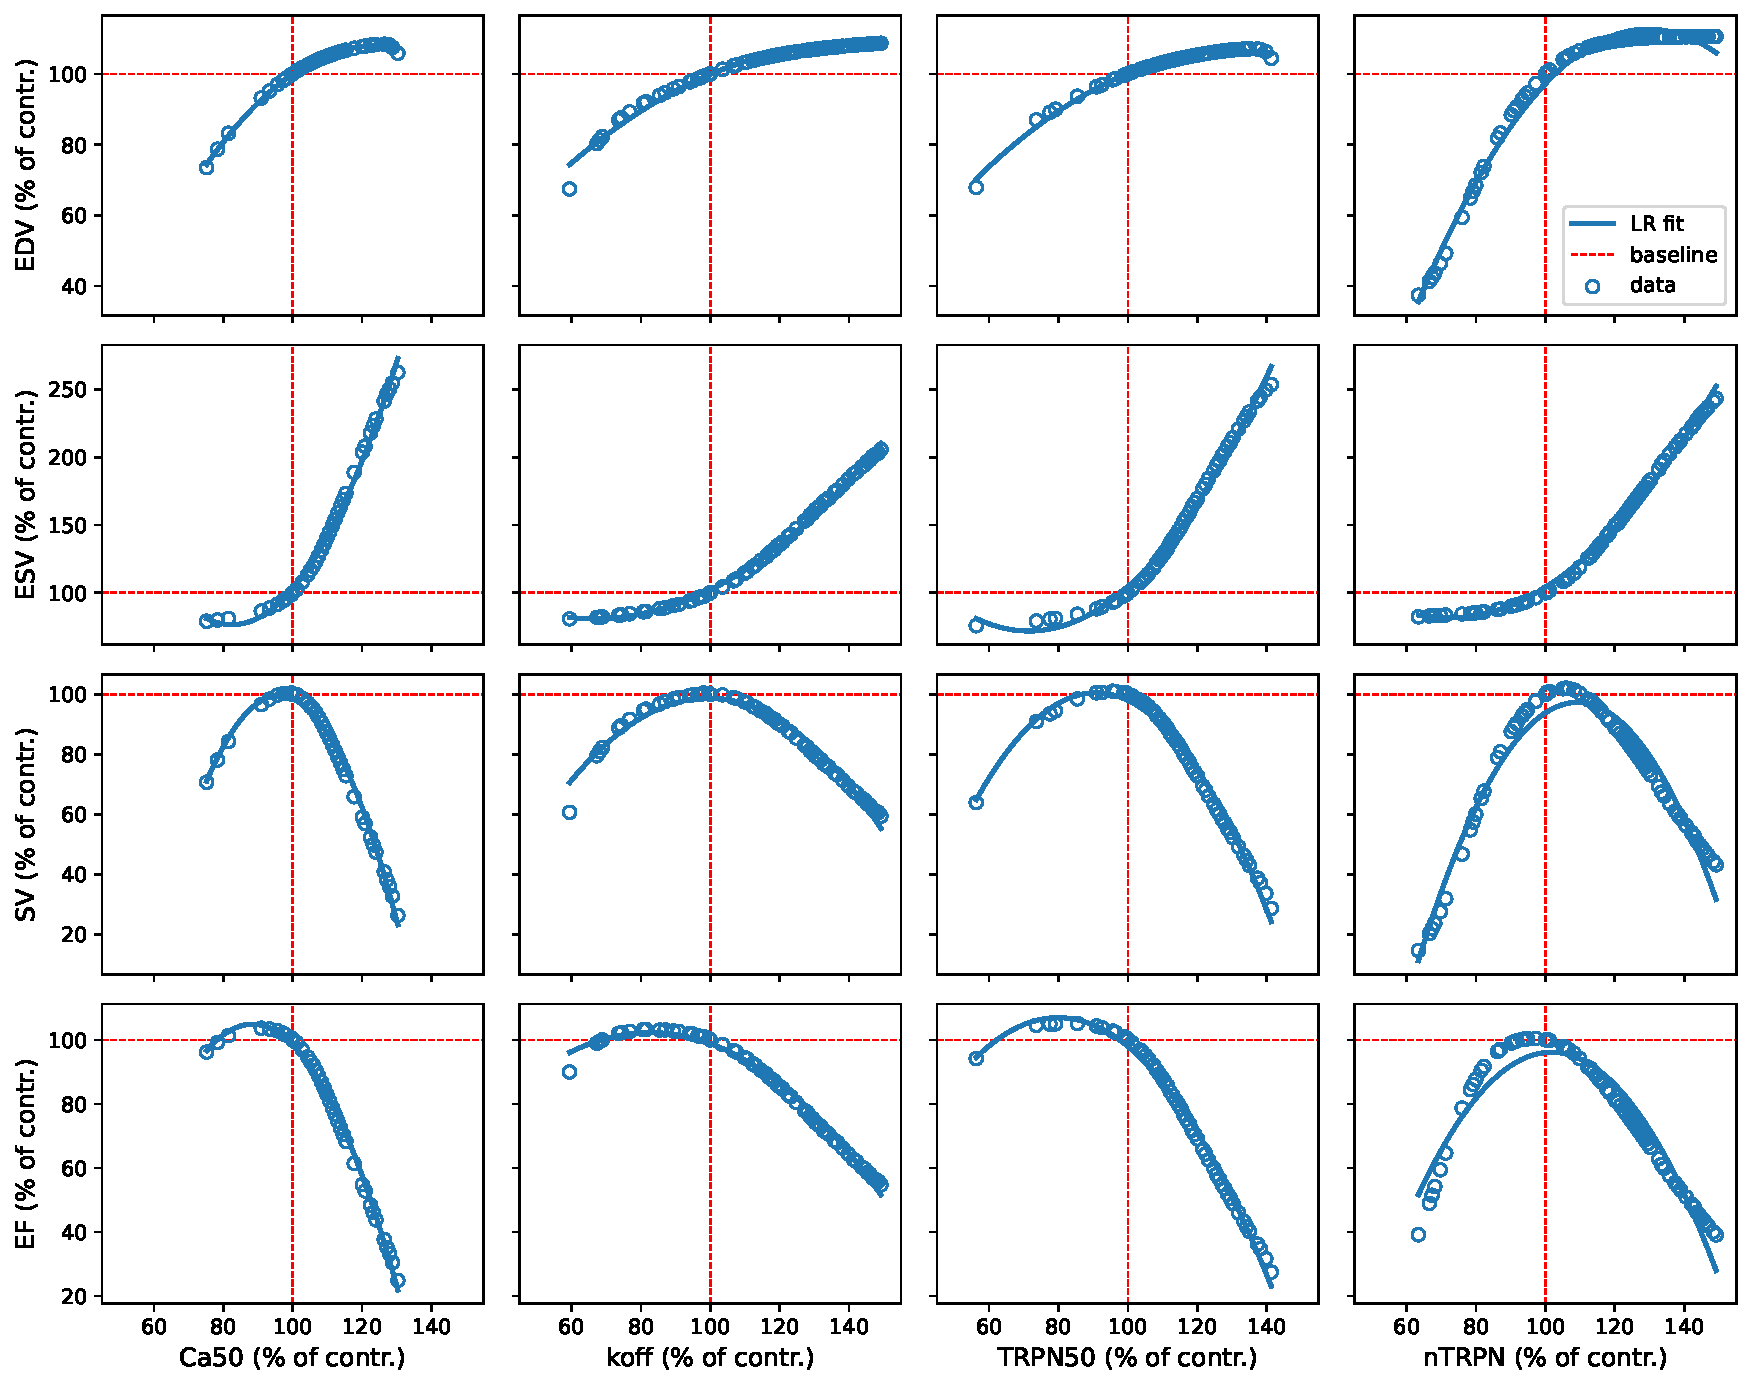
\includegraphics[width=\textwidth]{figures/chapter08/Fig1.pdf}
    \caption{The full $3$D biventricular rat heart contraction model is run at a fixed parameter set with only one parameter taking equally-spaced values in the $\pm\SI{50}{\percent}$ range of perturbation from its baseline value (vertical red dashed lines). The converging mechanics simulations' output PV loops are analysed to extract the corresponding EDV, ESV, SV and EF features' values (open blue dots), given as percentages from their baseline values (horizontal red dashed lines). The process is repeated separately for each parameter regulating the $\pCaf$ feature of the F-pCa curve. A linear regression (LR) model with second-order degree polynomials is fitted to the data (blue lines) for the sake of better visualising existing non-linear and non-monotonic relationships between the features and each of the parameters considered.}
    \label{fig:EFvsparamsnonmonotonic}
\end{figure}

\begin{figure}[h!]
    \myfloatalign
    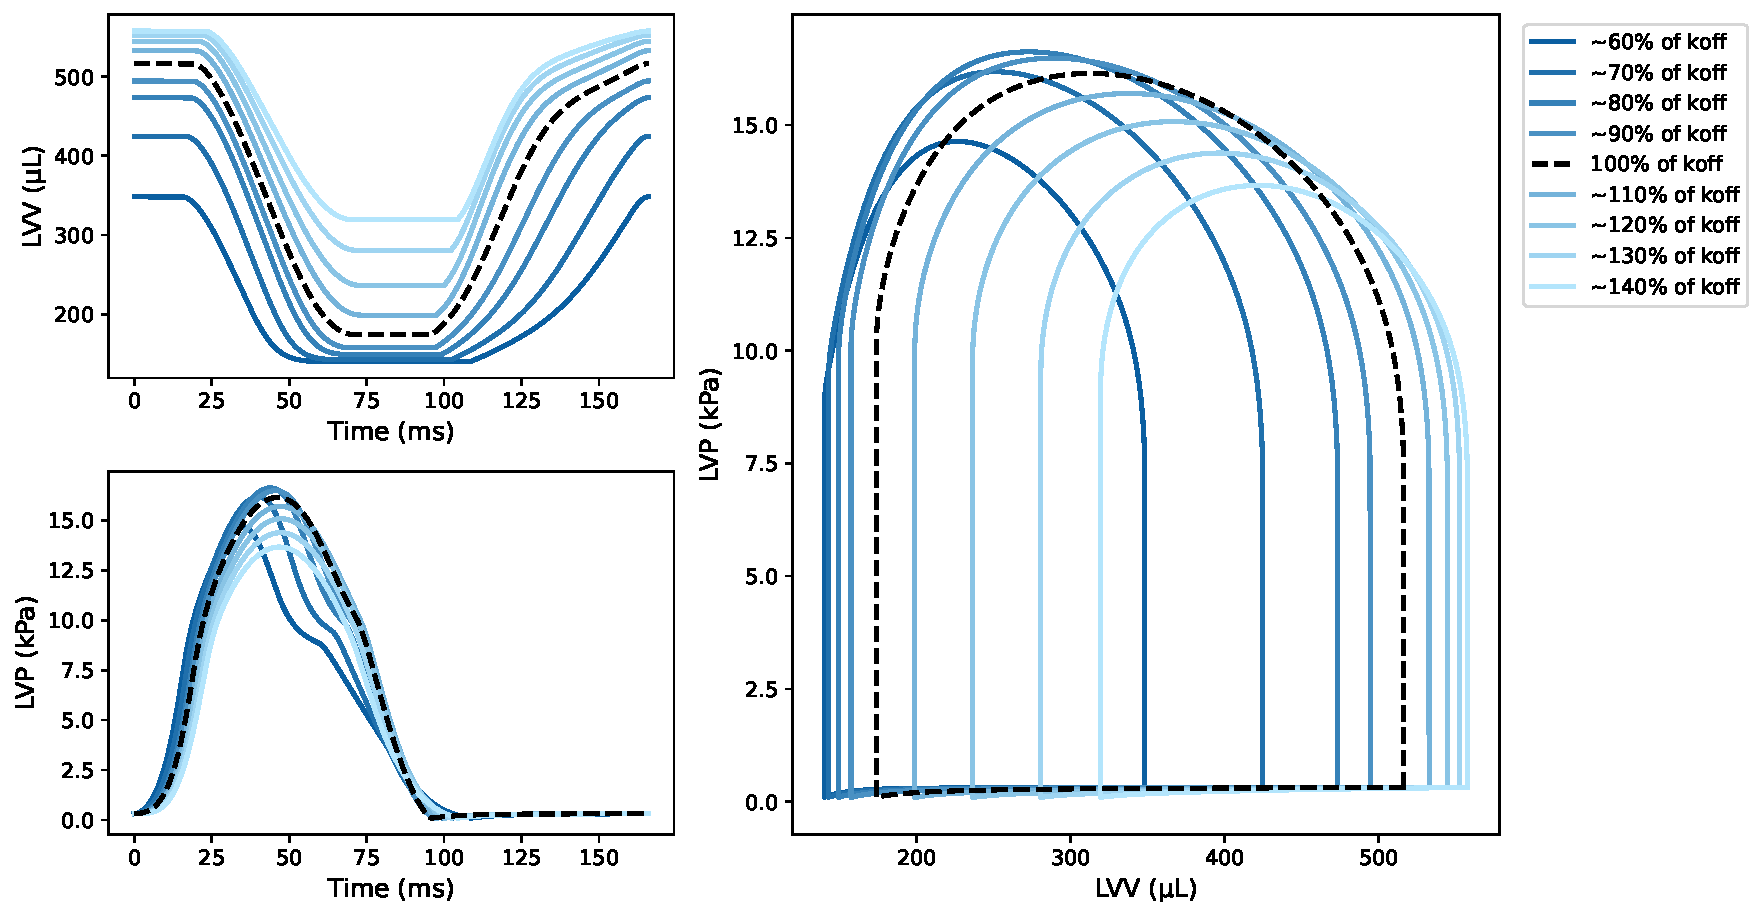
\includegraphics[width=\textwidth]{figures/chapter08/Fig2.pdf}
    \caption{The full $3$D biventricular rat heart contraction model is run at a fixed parameter set with only one parameter varying around its baseline value. Resulting LV volume and pressure transients and corresponding PV loops are plotted for some of the parameter values (full lines in blue variants), and compared to the reference parameter set mechanics solution (dashed black line). Example showing $\koff$ parameter variation in the range obtained as a $\pm\SI{40}{\percent}$ perturbation of its baseline value.}
    \label{fig:EFvskoff}
\end{figure}

\vspace{0.2cm}
We used pre-trained GPEs~\cite{Longobardi:2020} to evaluate how uncertainty in the simulator input (F-pCa curve-modulating parameters) affects the simulator output (LV features) via a GPE-based GSA. The regression accuracy of the employed GPEs is reported in the Supplementary material. The obtained GSA Sobol' sensitivity indices are displayed as donut charts in Figure~\ref{fig:gsarestr}. We can see that the reference thin filament $\Ca$ sensitivity ($\Caif$) is the most important parameter into explaining the total variance of EDV, ESV, SV and EF features. The second most important parameter is the degree of cooperativity of $\Ca$ binding to TnC ($\ntrpn$), followed by the fraction of bound $\Ca$-TnC complexes for half maximal cross-bridges activation ($\trpnf$) and the unbinding rate of $\Ca$ from TnC ($\koff$).

\begin{figure}[h!]
    \myfloatalign
    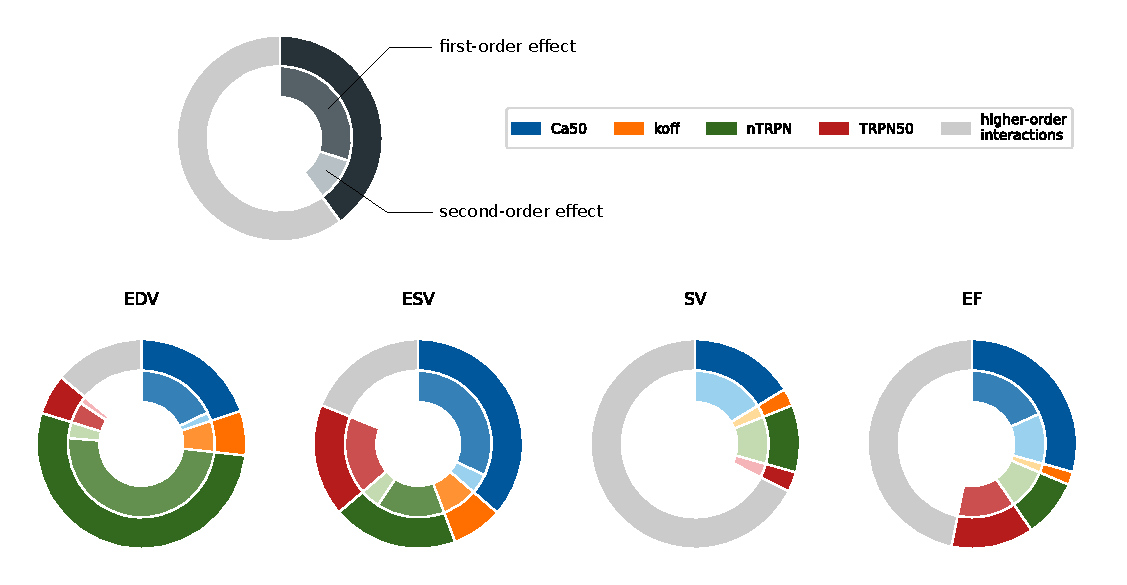
\includegraphics[width=\textwidth]{figures/chapter08/Fig3.pdf}
    \caption{The impact of $\pCaf$-modulating, sarcomere parameters on EDV, ESV, SV and EF organ-scale LV feature. The contribution of each parameter is represented by the sum of its first- and second-order effects. For each LV feature, higher-order interactions (up to the fourth order) are represented by the sum of all total effects minus the sum of all first- and second-order effects.}
    \label{fig:gsarestr}
\end{figure}


%
%
%
\subsection{$\pCaf$ changes are non-uniquely explained by sarcomere alterations: the one-parameter case}\label{sec:changespCa50result1}
We show that an observed change in $\pCaf$ can be caused by multiple different changes in sarcomere proprieties represented by model parameters. For each parameter $p_i,\,i=1,\,\dots,\,5$ of equation~\eqref{eq:pCa50params}, we report in Table~\ref{tab:alphavalues} the corresponding scaling coefficient $\alpha_i,\,i=1,\,\dots,\,5$ that would yield a shift of exactly $\Delta$ units in the $\pCaf$ value. This proves that an observed change in the F-pCa cannot be uniquely explained by a specific change in sarcomere properties. An example of $\pm\SI{2}{\percent}$ shift from a reference $\pCaf$ value is displayed in Figure~\ref{fig:2perclwrwshift}.

\begin{table}[h!]
    \myfloatalign
    \begin{tabularx}{\textwidth}{XX}
        \toprule
        \tableheadline{Parameter} & \tableheadline{Scaling coefficient $\boldsymbol{\alpha}$} \\
        \midrule
        & \\
        $\Caif$ & $10^{\Delta}$ \\ & \\
        $\kon$ & $10^{-\Delta\cdot\ntrpn}$ \\ & \\
        $\koff$ & $10^{\Delta\cdot\ntrpn}$ \\ & \\
        $\trpnf$ & $\dfrac{10^{\Delta\cdot\ntrpn}}{\trpnf(10^{\Delta\cdot\ntrpn}-1)+1}$ \\ & \\
        $\ntrpn$ & $\dfrac{\log\left(\frac{\koff}{\kon}\frac{\trpnf}{1-\trpnf}\right)}{\Delta\cdot\ntrpn+\log\left(\frac{\koff}{\kon}\frac{\trpnf}{1-\trpnf}\right)}$ \\ & \\
        \bottomrule
    \end{tabularx}
    \caption{By scaling each parameter $p_i$ by the corresponding $\alpha_i$ coefficient, the cellular contraction model simulates a $\pCaf$ value which is shifted by exactly $\Delta$ units from the reference value.}
    \label{tab:alphavalues}
\end{table}

\begin{figure}[h!]
    \myfloatalign
    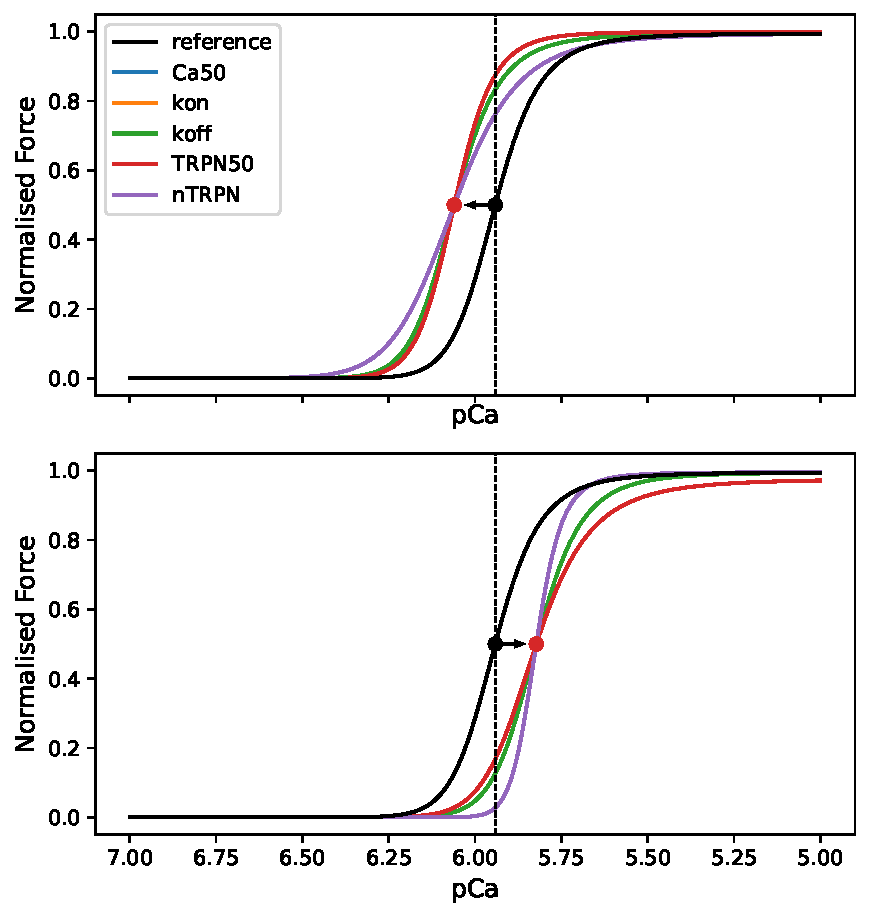
\includegraphics[width=0.6\textwidth]{figures/chapter08/Fig4.pdf}
    \caption{Different parameters can be individually perturbed to achieve the very same shift in the force-calcium relationship. Example showing $\SI{2}{\percent}$ leftwards (upper plot) and rightwards (bottom plot) shifts of the reference $\pCaf$ value. As $\trpnf$ and $\ntrpn$ also regulate the force-pCa curve's Hill coefficient (equation~\eqref{eq:h}), notice that for these two parameters the shift in the $\pCaf$ value is also affecting the curve's slope.}
    \label{fig:2perclwrwshift}
\end{figure}


%
%
%
\subsection{$\pCaf$ changes are non-uniquely explained by sarcomere alterations: the two-parameter case}\label{sec:changespCa50result2}
$\pCaf$ evaluation on $2$-parameter grids highlighted the presence of isolines, whose parameter points induce the same shifts in the $\pCaf$ feature value (Figure~\ref{fig:pca50isolines}A). This means that moving between any two points on two isolines will result in the same shift in $\pCaf$, demonstrating also in the two-parameter case the non-uniqueness of the F-pCa curve and a change in sarcomere properties.


%
%
%
\subsubsection{F-pCa curve mapping to LV function non-uniqueness}\label{sec:fpcatolvnonuniquemapping}
Parameter points inducing the same shifts in the $\pCaf$ feature value (isolines of Figure~\ref{fig:pca50isolines}A) are quantitatively linked to different EF feature values (Figure~\ref{fig:pca50isolines}B), showing that the mapping from F-pCa curve to LV function is not unique.

\begin{figure}[h!]
    \myfloatalign
    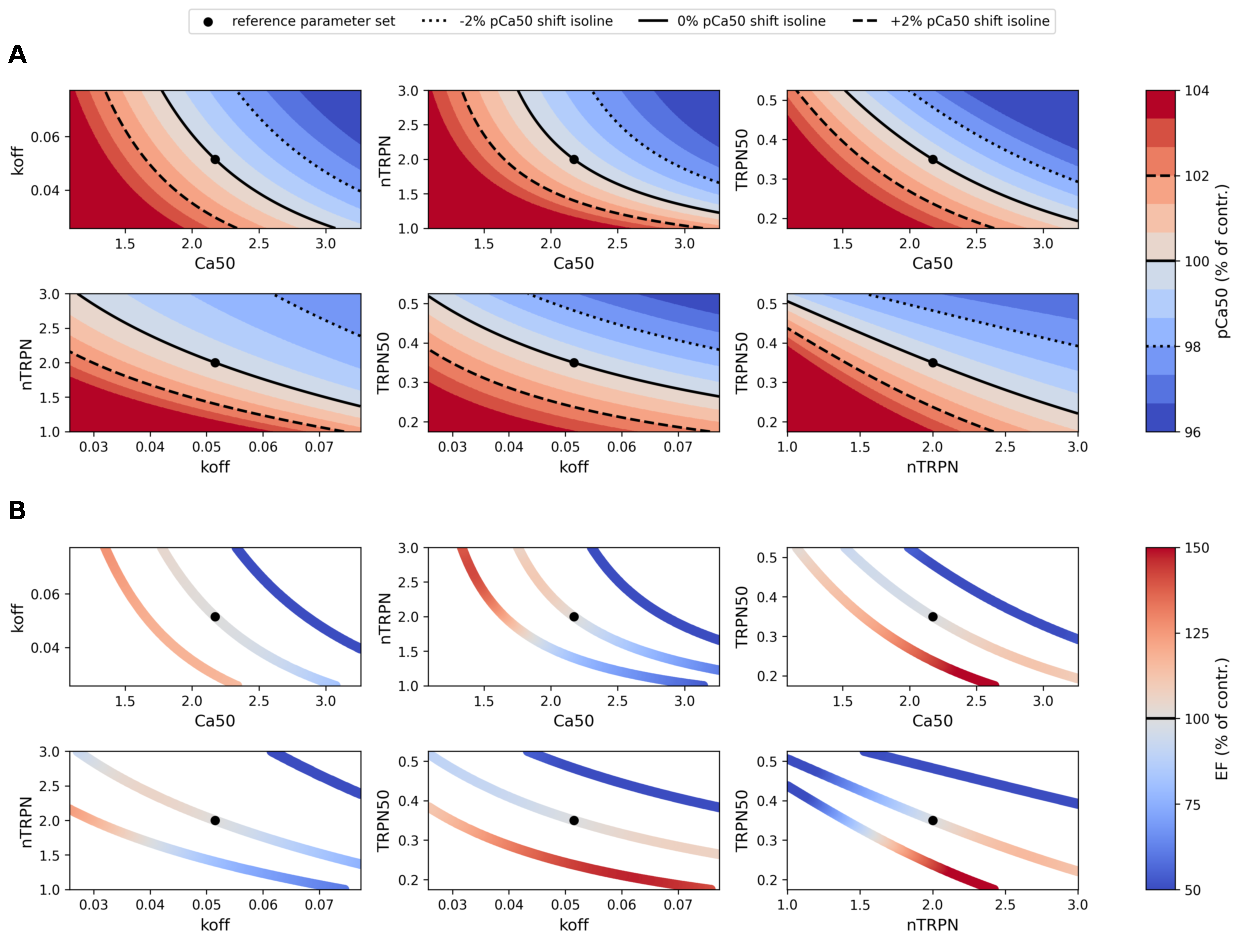
\includegraphics[width=\textwidth]{figures/chapter08/Fig5.pdf}
    \caption{For each pair of parameters regulating the $\pCaf$ feature of the F-pCa curve, a $2$D uniform grid is constructed using a $\pm\SI{50}{\percent}$ perturbation around the reference parameter set values (black dots). (A) The cell contraction model is then used to calculate the $\pCaf$ feature value at every parameter point of the grid, and each grid is plotted as a heat map with values given as percentages from the control $\pCaf$ value. Contour plots are finally added to highlight the presence of isolines, whose many different parameter sets induce the same shift ($-\SI{2}{\percent}$ dotted, $\SI{0}{\percent}$ full, $+\SI{2}{\percent}$ dashed black lines) in the control $\pCaf$ value. (B) Parameter points from the obtained isolines are mapped by the emulator into EF feature values. These values (given as percentages of the control EF value) are represented by different colour intensities used to colour each parameter point in the isolines, showing that parameters that share the same $\pCaf$ values are mapped to different EF values.}
    \label{fig:pca50isolines}
\end{figure}


%
%
%
\subsection{LV function changes are non-uniquely explained by sarcomere alterations}\label{sec:changesLVfunctionresult}
EF evaluation on $2$-parameter grids highlighted the presence of isolines, whose parameter points induce the same no-shift in the EF feature value (Figure~\ref{fig:EFisolines}A). This means that moving between any two points on each isoline will result in the same EF, demonstrating the non-uniqueness of the LV function and a change in sarcomere properties.


%
%
%
\subsubsection{LV function mapping to F-pCa curve non-uniqueness}\label{sec:lvtofpcanonuniquemapping}
Parameter points inducing the same no-shift in the EF feature value (isolines of Figure~\ref{fig:EFisolines}A) are quantitatively linked to different $\pCaf$ feature values (Figure~\ref{fig:EFisolines}B), showing that the mapping from LV function to F-pCa curve is not unique.

\begin{figure}[h!]
    \myfloatalign
    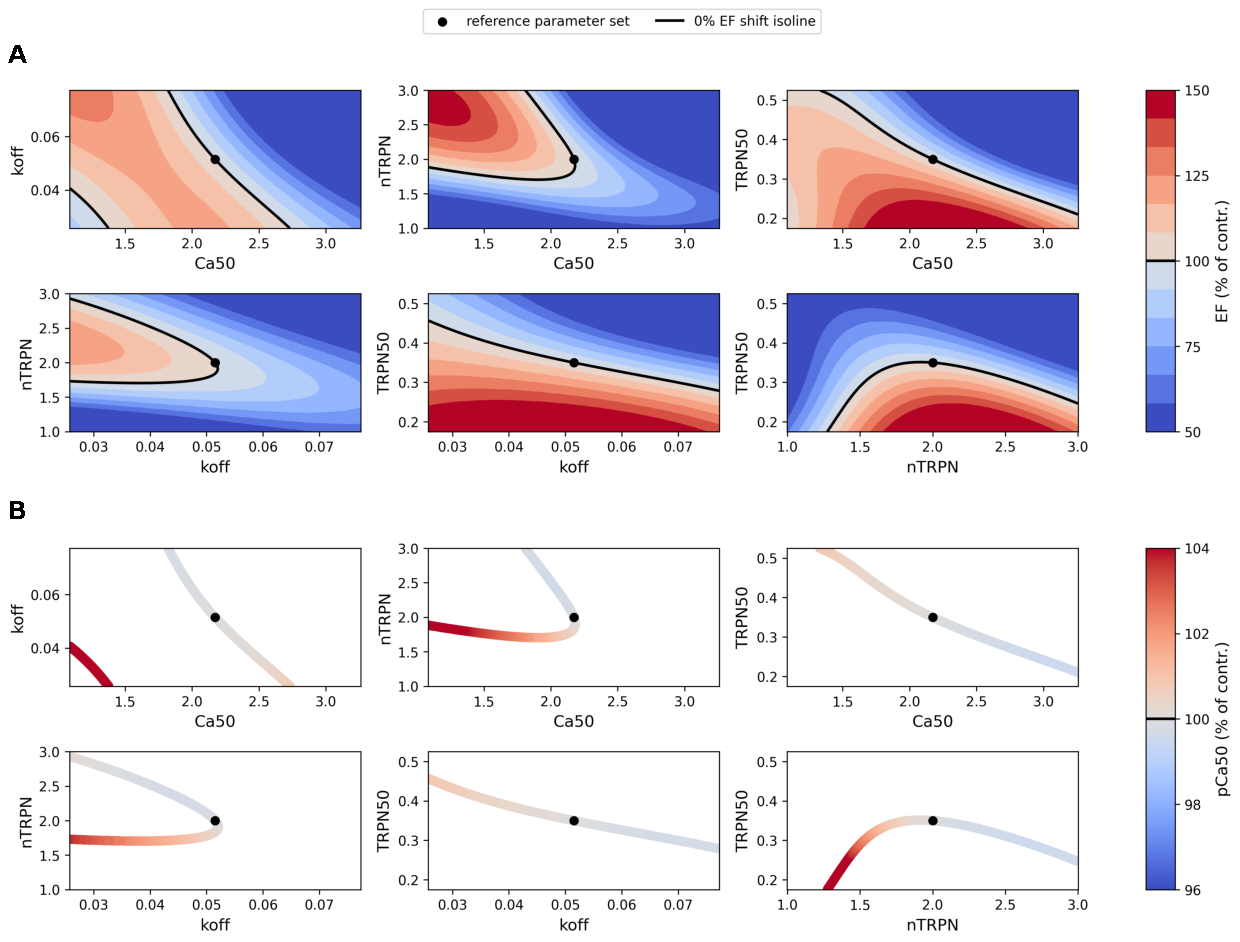
\includegraphics[width=\textwidth]{figures/chapter08/Fig6.pdf}
    \caption{For each pair of parameters regulating the $\pCaf$ feature of the F-pCa curve, a $2$D uniform grid is constructed using a $\pm\SI{50}{\percent}$ perturbation around the reference parameter set values (black dots). (A) A trained emulator is then used to predict the $\textrm{EF}$ feature value at every parameter point of the grid, and each grid is plotted as a heat map with values given as percentages from the control $\textrm{EF}$ value. Contour plots are finally added to highlight the presence of isolines (full black lines), whose many different parameter sets induce the same $\SI{0}{\percent}$ shift in the control $\textrm{EF}$ value. (B) Parameter points from the obtained isolines are mapped by the cell contraction model into $\pCaf$ feature values. These values (given as percentages of the control $\pCaf$ value) are represented by different colour intensities used to colour each parameter point in the isolines, showing that parameters that share the same $\textrm{EF}$ values are mapped to different $\pCaf$ values.}
    \label{fig:EFisolines}
\end{figure}


%
%
%
\subsection{F-pCa curve to LV function mapping and its inverse mapping are not unique}
In Sections~\ref{sec:changespCa50result1}--\ref{sec:changespCa50result2}, we proved that changes in the $\pCaf$ feature value are not uniquely caused by changes in sarcomere properties. In Section~\ref{sec:fpcatolvnonuniquemapping}, we also showed that changes in the EF feature value are not uniquely caused by changes in the $\pCaf$ value. Because of these two findings, we can state that observed changes in the F-pCa curve cannot be uniquely mapped to changes in the LV function.

\vspace{0.2cm}
At the same time, in Section~\ref{sec:changesLVfunctionresult} we proved that changes in the EF feature value are not uniquely caused by changes in sarcomere properties. In Section~\ref{sec:lvtofpcanonuniquemapping}, we also showed that changes in the $\pCaf$ feature value are not uniquely caused by changes in the $\textrm{EF}$ value. Because of these two other findings, we can state that observed changes in the LV function cannot be uniquely mapped to changes in the F-pCa curve.


%
%
%
\section{Discussion}\label{sec:ch8discussion}
\todo{this is Discussion copy-pasted from the paper: adapt it to thesis}

\noindent
In this study, we have made use of mathematical models to characterise the relationship between sarcomere properties and the LV contractile function in the healthy rat heart. We have highlighted the presence of complex nonlinearities, in particular we have demonstrated that the relationship between myofilaments' features (e.g. $\Caif$) and PV loop characteristics (e.g. EF) is non-monotonic. As these sarcomere properties also define the steady-state force-calcium relationship in the cardiac muscle, we extended this result in terms of shifts in the F-pCa curve that are normally examined when experimentally assessing the effect of sarcomere-targeting pharmacological compounds. We have therefore provided both analytical and simulation study evidence that alterations in the F-pCa curve can cause very different changes in whole heart function. At the same time, we have shown that observed changes in the LV function cannot be attributed to a unique modification in sarcomere properties. Although we characterised the LV function using the EF feature, the obtained results more generally hold true for many other clinically relevant indexes of LV both systolic and diastolic function, including isovolumetric relaxation time, peak pressure and maximum rates of pressure rise and decay (see Supplementary material for more details).

The performed GSA interpreted the variability of EDV, ESV, SV and EF in terms of the uncertainty in F-pCa curve-modulating sarcomere parameters, and it emphasised the importance of the $\Ca$ sensitivity into affecting these PV loop characteristics. A deeper insight can be gained if we look at higher-order interactions' effects. Although these are present for all the four LV features considered, they are remarkably high only for the SV and EF features, explaining more than half of the total variance for SV and almost half of the total variance for EF. We can notice that for the EDV and ESV features higher-order interactions' effects are instead small, and dominating effects are mostly of the first-order type. Conversely, for the SV and EF features where higher order interactions' effects are high, dominating lower-order effects are mostly of the second-order type. All these considerations can be summarised by stating that although it is possible to interpret changes in terms of the individual contribution of parameters for the EDV and ESV features, this is not the case for SV and EF features. In this sense, it is more the joint effect of the whole sarcomere to determine the LV function rather than single myofilament components.

Indications from the GSA coupled with the information of F-pCa curve vs. LV function non-monotonicity shed a new light on the problem of interpreting pharmacological interventions' effects on the F-pCa curve in terms of the desired effects on whole-heart function. This concept is illustrated via the schematic in Figure~\ref{fig:schematic}, which highlights existing feedback mechanisms that regulate contraction in the heart. Modulation of the $\Ca$ transient can directly affect the active tension which is generated within the sarcomere, and alteration of the sarcomere generated force will eventually affect the PV loop. As the force-volume relationships at the end-diastolic and end-systolic pressures are fixed, sarcomere interventions that aim at shifting the F-pCa might cause no change in LV contractile function. For this reason, treatment strategies should aim at altering both the end-systolic and end-diastolic force-volume relationships to yield an effect on the PV loop.

\begin{figure}[h!]
    \myfloatalign
    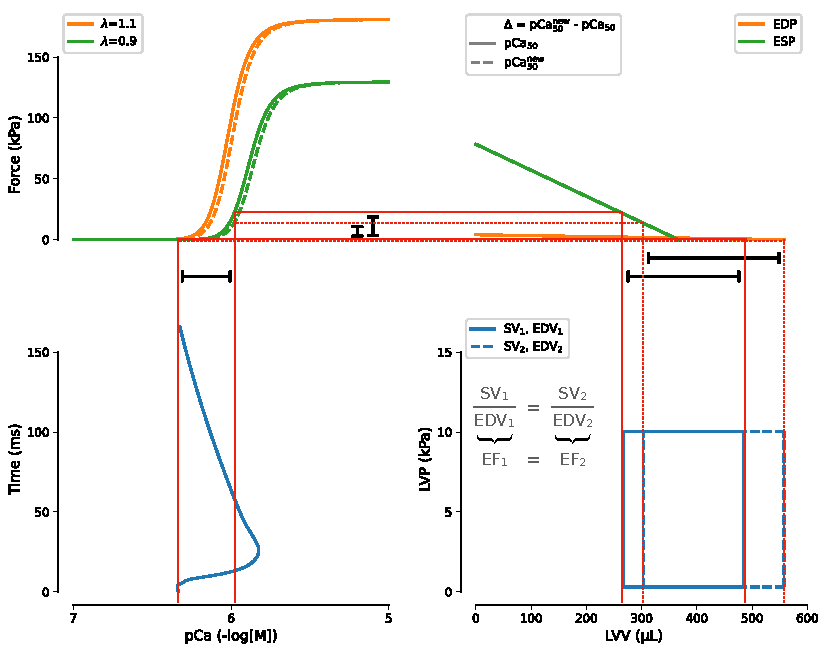
\includegraphics[width=\textwidth]{figures/chapter08/Fig7.pdf}
    \caption{Force-LV volume curves at the end-diastolic and end-systolic pressures (top right, orange and green lines) can be separately manipulated to modulate the LV contractile function. However, interventions on calcium transient (bottom left, blue line) and sarcomeric generated force (top left, orange and green full lines) both reflect into modifications of the former curves, which in turns causes modification of the PV loop (bottom right, blue full line). Pharmacological modulations on the sarcomere might cause a shift of the force-calcium relationship (top left, orange and green dashed lines). However, this will preserve the EF (bottom right, blue dashed line) without improving LV contractile function, which was the desired outcome of the performed sarcomeric intervention.}
    \label{fig:schematic}
\end{figure}

\vspace{0.2cm}\noindent
\todo{this is Limitations copy-pasted from the paper: adapt it to thesis}

\noindent
This work has different limitations. First, the used cellular contraction model is only a simplified representation of the sarcomere, without a detailed mechanistic description of its components. Specifically, the cross-bridge kinetics is described by a two-state model where the strongly-/weakly-/un-bound states are collapsed into a single state. While more detailed models exist~\cite{Land:2015}, their parameters are not necessarily constrained using experimental data due to difficulties in measuring subcellular processes, and are not easily integrable into multi-scale whole-organ simulations. The used model is still able to recapitulate all the main sarcomere processes including the length and velocity dependencies. Second, the employed $3$D healthy rat heart contraction mechanics model that incorporated the cellular contraction model does not account for the pericardium and the atria and is not a closed loop system, being more close to an \textit{ex-vivo} rather than an \textit{in-vivo} rat heart model. All these factors could play a role in constraining the heart contraction mechanics, however we have previously~\cite{Longobardi:2021} demonstrated that this model is still able to capture and reproduce pharmacological interventions' effects at the sarcomere level in the form of F-pCa curve changes and map those to whole heart behaviour, consistently with literature preclinical experimental evidence. Third, the use of emulators adds an additional layer of uncertainty in modelling the LV function, since emulators are probabilistic surrogates of the simulator, which is already an \textit{in-silico} representation of the real world biological system. However, the speedup that we gain by using emulators which enables efficient identification of the sarcomere parameters which play a key role in determining the LV function at whole-organ overcomes by far the slight loss in quantitative accuracy when making predictions. This is because the focus was on mapping changes from reference values in the F-pCa curve to changes from reference values in the LV function and vice-versa, rather than mapping absolute values.


%
%
%
\section{Summary}\label{sec:ch8summary}
\todo{this is Conclusion copy-pasted from the paper: adapt it to thesis.} We have used a biophysically detailed mathematical model of a healthy rat heart contraction to quantitatively map sarcomere properties to whole heart function. Using this mapping, we demonstrated that the relationship between F-pCa curve and LV function is non-linear and non-monotonic. This results in the non-interpretability of observed changes in the LV function in terms of unique sarcomere modulations, which highlights the need for muscle experimental findings to be put into a broader context where not only the $\pCaf$ and Hill coefficient, but also active and passive force, length and velocity dependencies, calcium transient and boundary conditions are analysed.